% beamfs v3 technical report
% Author: Aurelien DESBRIERES
% License: CC-BY-4.0
% Build: python3 scripts/tables.py && latexmk -lualatex paper.tex
% Every number quoted in the text comes from generated/numbers.tex,
% written by scripts/tables.py from data/derived/*.csv, itself written
% by scripts/extract.py from the signed run records.

\documentclass[10pt,conference,a4paper]{IEEEtran}

% LuaLaTeX font stack (as v2)
\usepackage{fontspec}
\usepackage{amsmath}
\usepackage{mathtools}
\usepackage{unicode-math}
% IEEEtran sets section titles in small caps: Latin Modern keeps them
% in a separate family.
\setmainfont{Latin Modern Roman}[SmallCapsFont={lmromancaps10-regular.otf}]
\setsansfont{Latin Modern Sans}
\setmonofont{Latin Modern Mono}
\setmathfont{Latin Modern Math}

% Tables
\usepackage{booktabs}
\usepackage{tabularx}
\usepackage{multirow}

% Figures
\usepackage{graphicx}
\usepackage{tikz}
\usetikzlibrary{positioning,shapes,arrows.meta,calc,decorations.pathreplacing}

% Code
\usepackage{listings}
\lstset{
  basicstyle=\ttfamily\footnotesize,
  breaklines=true,
  showstringspaces=false,
  columns=fullflexible,
}

% URLs and long hashes
\usepackage{xurl}
\usepackage{seqsplit}

% Bibliography (as v2)
\usepackage[backend=biber,style=ieee,sorting=none,maxbibnames=5,
            doi=true,url=true,isbn=false]{biblatex}
\addbibresource{refs.bib}

\usepackage{hyperref}
\hypersetup{
  colorlinks=true,
  linkcolor=blue!50!black,
  citecolor=blue!50!black,
  urlcolor=blue!50!black,
  pdftitle={beamfs v3: an EM-resilient Linux filesystem under read-path fault injection, with an audit of the injector},
  pdfauthor={Aurelien Desbrieres},
  pdfsubject={Filesystem; electromagnetic resilience; Reed-Solomon; Linux kernel; fault injection},
  pdfkeywords={beamfs, electromagnetic resilience, Reed-Solomon, filesystem, Linux kernel, emufi, xfstests, fault injection},
}
\usepackage[capitalize,noabbrev]{cleveref}

\usepackage{microtype}
\usepackage{xspace}
\usepackage{enumitem}
\usepackage{placeins}
\setlist{nosep,leftmargin=1.5em}

% Generated by scripts/tables.py from data/derived/*.csv. Do not edit.
\newcommand{\commitBenchTwo}{661e8aa}
\newcommand{\manifestShaTwo}{57f2335a9fe82288307b1214b0d6975919d4f13549f2d2e4c89cf5a96e8c6e00}
\newcommand{\manifestNameTwo}{manifest-20261005T191045Z.json}
\newcommand{\commitBenchThree}{60155f3}
\newcommand{\manifestShaThree}{506e0da692874722a70ec0e8196e6b91a63560478daf3837e5ae18340e711755}
\newcommand{\manifestNameThree}{manifest-20261008T064257Z.json}
\newcommand{\commitBenchFour}{607716e}
\newcommand{\manifestShaFour}{15e9042d1e5dd57621162c31d756bfcbcf003772ae28f34329b5f16c8236e789}
\newcommand{\manifestNameFour}{manifest-20261008T081801Z.json}
\newcommand{\commitBeamfs}{1bf151d}
\newcommand{\commitBeamfsFull}{1bf151d9f530b44d20837db62ccdeaa7a6c7c785}
\newcommand{\commitYocto}{9d43172}
\newcommand{\imageSha}{1d60a1be893fa8eae92463082181d77be207393a3a7e18ffff7cc60183963e62}
\newcommand{\rcRunFour}{0}
\newcommand{\moduleLines}{17\,348}
\newcommand{\moduleFiles}{19}
\newcommand{\sweepXfullSha}{dec773163aa0edc008e95cf4eb8f30a77edaa29b976b44eb3fd782b6562b9a00}
\newcommand{\sweepXfullName}{sweep-1790972412.results}
\newcommand{\sweepAfullSha}{8b86f2562183fc36808a8ff500819d30240045dfaf0c2824aa6550878bd85b78}
\newcommand{\sweepAfullName}{sweep-1791190821.results}
\newcommand{\sweepXsoloSha}{c0c985526f482af4b93e9374df5dbd08a79e5b4fdcb50dc1d5a62355ad5a7d39}
\newcommand{\sweepXsoloName}{sweep-1791196367.results}
\newcommand{\sweepAsoloSha}{9130579830953f817eed7814aa55e9784613e575b3790ccb4a62586275193b37}
\newcommand{\sweepAsoloName}{sweep-1791214142.results}
\newcommand{\xfsXsoloSeconds}{2\,317}
\newcommand{\xfsAsoloSeconds}{11\,483}
\newcommand{\snapshotSha}{6f2e4a77fea51ca737b0bdfc3b7892e730c2041ac57ab7213fa8a824a98b9667}
\newcommand{\snapshotFiles}{2532}
\newcommand{\extractSha}{516f58c0162da48b99bbb10dad79ba873d028c5916df7fe8f04b860e64ef4046}
\newcommand{\figuresSha}{a18e643c9b20476c90e1776300b8c17f7797043d6c22c3b3ef572d35ed0effa1}
\newcommand{\tablesSha}{730219724e38b80dc7aa3ef48d5abf2973dd8b3a7541db7ce3e1e2cbf2d92f36}
\newcommand{\xfsTotal}{734}
\newcommand{\xfsGenericAuto}{731}
\newcommand{\xfsSharedAuto}{3}
\newcommand{\xfsXRan}{122}
\newcommand{\xfsXPass}{122}
\newcommand{\xfsXFail}{0}
\newcommand{\xfsXNotrun}{612}
\newcommand{\xfsXNoverdict}{0}
\newcommand{\xfsXNrFeature}{511}
\newcommand{\xfsXNrEnv}{98}
\newcommand{\xfsXNrScope}{3}
\newcommand{\xfsXFailList}{none}
\newcommand{\xfsARan}{123}
\newcommand{\xfsAPass}{122}
\newcommand{\xfsAFail}{1}
\newcommand{\xfsANotrun}{611}
\newcommand{\xfsANoverdict}{0}
\newcommand{\xfsANrFeature}{511}
\newcommand{\xfsANrEnv}{97}
\newcommand{\xfsANrScope}{3}
\newcommand{\xfsAFailList}{generic/476}
\newcommand{\xfsXpass}{122}
\newcommand{\xfsApass}{122}
\newcommand{\xfsAfullSeconds}{14\,388}
\newcommand{\xfsAfullVerdict}{FAIL}
\newcommand{\xfsNotrunDiffer}{1}
\newcommand{\xfsNotrunDifferList}{generic/317}
\newcommand{\xfsGroups}{42}
\newcommand{\xfsXtag}{sweep-1791491243}
\newcommand{\xfsXkernelSha}{837c86337113b56f4a1fc81221cdf617ec19c6bd0b53845af2a038668f6ae84f}
\newcommand{\xfsXtaintStart}{0}
\newcommand{\xfsXtaintEnd}{0}
\newcommand{\xfsXfullSeconds}{2\,653}
\newcommand{\xfsXkernLogs}{734}
\newcommand{\xfsXtreeLogs}{734}
\newcommand{\xfsSupFullSeconds}{1\,883}
\newcommand{\xfsSupDone}{603}
\newcommand{\xfsSupTag}{sweep-1791470226}
\newcommand{\xfsSupVerdictsSha}{d954c2092c1a1313b4a268eb965b55717ca1506bcea805a359ba529f55566541}
\newcommand{\xfsXmetaSha}{86d05bbd107cbf1f862470a0ad0e7cad54ebaf15bd0e6389848b4e3141726d76}
\newcommand{\xfsXverdictsSha}{f1f450f0d5dc30e37e3702b1f682ca107b511ad6a41e2f39fb595bee9e20907c}
\newcommand{\xfsAcheckOutputs}{733}
\newcommand{\xfsXMkfsSha}{6843a47cb41ff07c378c8db038fd1560b33169ad72adae7a61dd7fa45b4467a1}
\newcommand{\xfsXMkfsVersion}{0.1.5}
\newcommand{\xfsXFsckSha}{ba772535ea050fb7e5217fcb9fe97839b0e9b27ce10628c2ab124c7870432fb8}
\newcommand{\xfsXFsckVersion}{0.1.8}
\newcommand{\featXfstests}{0x7a000}
\newcommand{\imageXSha}{af9d860bbc94127cd842c2a1bd265265c160e3628a1882ea105b20fb6210e08e}
\newcommand{\kernelXSha}{837c86337113b56f4a1fc81221cdf617ec19c6bd0b53845af2a038668f6ae84f}
\newcommand{\kernelASha}{a15840c81b0d6ec74fd80145b8b8da245216e1fa055a4debe2c8cb2fd21a096a}
\newcommand{\srcTrees}{6}
\newcommand{\mfBeamfsMaxFlips}{265}
\newcommand{\mfExtFourFlipsMin}{1}
\newcommand{\mfExtFourFlipsMax}{1}
\newcommand{\mfExtFourOutcome}{silent corruption}
\newcommand{\mfExtThreeFlipsMin}{2}
\newcommand{\mfExtThreeFlipsMax}{3}
\newcommand{\mfExtThreeOutcome}{silent corruption}
\newcommand{\mfBtrfsFlipsMin}{2}
\newcommand{\mfBtrfsFlipsMax}{2}
\newcommand{\mfBtrfsOutcome}{read refused}
\newcommand{\mfBeamfsHighTwo}{265}
\newcommand{\mfBeamfsMidTwo}{20}
\newcommand{\mfBeamfsHighThree}{265}
\newcommand{\mfBeamfsMidThree}{22}
\newcommand{\mfBeamfsHighFour}{262}
\newcommand{\mfBeamfsMidFour}{33}
\newcommand{\clRunFourIntact}{9}
\newcommand{\clRunFourNoFlip}{3}
\newcommand{\clRunThreeRefusedFlips}{263}
\newcommand{\kernLines}{60}
\newcommand{\kernMaxPerDecode}{2}
\newcommand{\unionMax}{3}
\newcommand{\dtPairMaxMicro}{183}
\newcommand{\dtOtherMinMilli}{2.51}
\newcommand{\ambiguousHigh}{0}
\newcommand{\featIncompat}{0x7a100}
\newcommand{\indHits}{5}
\newcommand{\indSlots}{489 (run 2), 355 (run 2), 511 (run 3), 338 (run 3), 373 (run 4)}
\newcommand{\flipsAnalysed}{867}

% The filesystem's name, in roman like ext4 or btrfs: IEEEtran sets the
% abstract in bold and captions in small caps, which Latin Modern Mono
% does not have.
\newcommand{\bfs}{beamfs\xspace}
% \seqsplit needs the digits themselves, not the macro that holds them.
\newcommand{\hash}[1]{\texttt{\expandafter\seqsplit\expandafter{#1}}}
\newcommand{\apprepro}{\hyperref[sec:repro]{the appendix}}
% A statement not yet confirmed on the station. scripts/check-paper.sh
% refuses a release build while one remains.
\newcommand{\verify}[1]{\textcolor{red}{#1}}

% =====================================================================
\title{\large\bfseries beamfs v3:\\
       An EM-Resilient Linux Filesystem\\
       under Read-Path Fault Injection,\\
       with an Audit of the Injector\\
       \small\itshape Technical Report, Version 3}

\author{%
  \IEEEauthorblockN{Aur\'elien Desbri\`eres, independent researcher}
  \IEEEauthorblockA{\href{https://orcid.org/0009-0002-0912-9487}{ORCID:~0009-0002-0912-9487} \quad
    \texttt{aurelien@hackers.camp}}
}

\begin{document}
\raggedbottom
\maketitle

\begin{abstract}
\bfs is a Linux filesystem that stores every data block as a capsule of
sixteen interleaved Reed-Solomon RS(255,239) codewords, decodes on every
read, and refuses a read it cannot vouch for. This report measures
\bfs 0.1.26 (commit \commitBeamfs) on Linux 7.3-rc5. Of the
\xfsTotal{} tests of the xfstests auto group, all \xfsXRan{} that ran
on x86-64 passed, and \xfsAPass{} of the \xfsARan{} that ran on
aarch64; xfstests declined the others, most of them for features \bfs
does not implement, and these are counted apart, not as passes. Under
single-bit upsets injected into read bios by the emufi injector, on a
four-node aarch64 cluster and on USB flash media, \bfs never returned
wrong data: it returned the correct file in every exercised case but
one, absorbing up to \mfBeamfsMaxFlips{} flips during one read of a
256\,KiB file, and in that one refused the read, after a flip in an
indirect pointer. In the same runs ext4 and ext3 returned silently corrupted
data after \mfExtFourFlipsMax{} and \mfExtThreeFlipsMin{} to
\mfExtThreeFlipsMax{} flips respectively, and btrfs refused the read.
We audit the injector itself. On this kernel emufi 0.8.1 logs one of its
two read hooks one bio before the block it flips; reconstructing the hook
of every flip explains all \kernLines{} corrections the kernel reported
and bounds the load at \kernMaxPerDecode{} erroneous symbols per codeword
and per decode, against eight correctable. The campaign therefore
exercises detection and correction end to end, not the correction limit.
Redundancy (btrfs DUP data, ZFS with two copies) also returns
correct data, for a full copy; \bfs does it on one medium for 7\,\% of
capacity, while its indirect pointers, in the default configuration, are
less protected than ext4's checksummed extent blocks. We set out what
\bfs brings, what it costs, and what v4 takes on.
Scope, after the project's normative statement: \bfs is designed against
Family~A perturbations (stochastic electromagnetic single-bit and
multi-bit upsets, aging silicon bit-rot, environmental radiation,
rowhammer-class single-cell flips); Family~B perturbations (adversarial
bursts exceeding 256 octets per sub-block, IEMI at scale, voltage-glitch
attacks at scale) are not claimed. This report measures a subset of
Family~A. Every number in it is generated from signed run records and
cross-checked before typesetting.

\end{abstract}

\begin{IEEEkeywords}
Electromagnetic resilience, filesystem, Reed-Solomon, Linux kernel,
fault injection, emufi, xfstests, single-event upset, reproducibility
\end{IEEEkeywords}

\section{Introduction}\label{sec:intro}

A filesystem trusts the bytes a read brings back. Between the medium and
the page cache those bytes cross a controller, a bus, DMA buffers and
caches, any of which can flip a bit: soft errors in commercial silicon
are a measured fact~\cite{baumann2005}, and they matter most where
hardware is commercial and the environment is not. Memon et
al.~\cite{memon2025tr,memon2025arxiv} irradiated commercial systems on
chip running Linux with 20 to 58\,MeV protons and found that, on an
i.MX~8M~Plus running ext4 on eMMC, filesystem faults and storage-driver
errors accounted for 90\,\% of the observed failures, up to journal
aborts and read-only remounts~\cite{memon2025arxiv}. Conventional
filesystems either do not check file data (ext4, ext3) or check it and,
holding a single copy, refuse the read (btrfs); they return the data the
application wrote only from a second copy of
it~\cite{btrfsautorepair,zfschecksums}.

\bfs~\cite{beamfsimpl} is a Linux filesystem built to return it, or to
refuse. Every data block is a \emph{capsule} of sixteen interleaved
RS(255,239) codewords~\cite{reed1960,macwilliams1977}; every read decodes
it; a block beyond correction fails the read with an error instead of
handing back wrong bytes. \bfs descends from FTRFS~\cite{fuchs2015ftrfs}
through an RFC posted in April 2026~\cite{ftrfsrfc} and two earlier
reports~\cite{desbrieres2026ftrfs,desbrieres2026beamfsv2}.
\Cref{sec:ftrfs} explains why it is a new filesystem rather than a
revision of FTRFS.

\paragraph*{What this report adds}
\begin{enumerate}
\item A measured \bfs 0.1.26: of the \xfsTotal{} tests of the xfstests
  \texttt{auto} group, all \xfsXRan{} that ran on x86-64
  passed, and \xfsAPass{} of the \xfsARan{} that ran on aarch64; the
  tests xfstests declined, mostly for features \bfs does not implement,
  are counted and classified, not passed (\cref{sec:xfstests}).
\item A comparison with ext4, ext3, btrfs and squashfs under emulated
  single-bit upsets on the read path, replicated over three runs, and a
  four-node cluster campaign (\cref{sec:multifs,sec:cluster}).
\item An audit of the injector. emufi 0.8.1~\cite{desbrieres2026emufi}
  logs one of its two read hooks one bio early on this kernel. We locate
  the cause in the kernel source, reconstruct the hook of every flip,
  and check the reconstruction against the kernel's own correction log
  (\cref{sec:injector}).
\item A fail-closed event on an indirect block, explained from the code,
  and the residual it exposes (\cref{sec:indirect}).
\item A parallel with the proton campaign of Memon et al., including what
  that work reports about the hardware it irradiated (\cref{sec:memon}).
\item A positioning of \bfs against redundancy, with its costs and
  where it is weaker today (\cref{sec:brings}), and the work the next
  version takes on (\cref{sec:v4}).
\item A reproducibility record in which every number of the text is
  generated from GPG-signed run manifests and frozen by hash
  (\apprepro).
\end{enumerate}

\paragraph*{What changed since v2}
The v2 report~\cite{desbrieres2026beamfsv2} is superseded on five
points. (i)~Data blocks are now interleaved capsules
(\cref{sec:capsule}); v2 described the alternating layout. (ii)~v2 stated
that a corrected block is written back to the medium on read; in
0.1.26 the read path corrects into a private copy and does not write
back, on-disk repair being left to the background scrubber
(\cref{sec:readpath}). (iii)~The module is no longer 2\,198 lines: it is
\moduleLines{} lines of C and headers at \texttt{\commitBeamfs}, beyond the
5\,000-line audit target v2 quoted. (iv)~Injection moved from RadFI~\cite{desbrieres2026radfi} to
emufi. (v)~Validation is the xfstests \texttt{auto} group, test by test,
on two architectures.

\section{From FTRFS to beamfs}\label{sec:ftrfs}

FTRFS~\cite{fuchs2015ftrfs} proposed a filesystem for the on-board
memory of spacecraft: checksums, forward error correction and memory
protection over a small radiation-exposed store. Its Linux realisation,
posted as an RFC in April 2026~\cite{ftrfsrfc} and described in the
FTRFS v1 report~\cite{desbrieres2026ftrfs}, inherited the concept and
its limits. Each limit below is conceptual, not a missing feature: it
follows from the threat model or from the place error correction holds
in the design, which is why \bfs is a new filesystem with its own
on-disk format rather than a further FTRFS revision.
\Cref{tab:ftrfs} sets them side by side.

\paragraph*{Threat model}
FTRFS assumes radiation-induced upsets arriving as independent events at
a low constant rate, the Poisson regime of space radiation. It says
nothing about correlated events, bursts, or a deliberate attacker. The
soundness theorem of the first \bfs report was stated under that model;
fault injection falsified it, and v2 withdrew it~\cite{desbrieres2026beamfsv2}.
\bfs states two families of perturbation, claims one, and says which
(\cref{sec:scope}).

\paragraph*{Where correction sits}
In FTRFS, Reed-Solomon protects metadata and a CRC guards each block;
the decoder runs once a CRC has failed, and the RFC shipped the encoder
only~\cite{ftrfsrfc}. File data, the part an application reads back,
had no correction at all, and a CRC that is itself hit can mask or
invent a failure. In \bfs every data block is encoded, and the decoder
runs on every read whatever any checksum says (\cref{sec:readpath}).

\paragraph*{Scale}
The FTRFS allocation bitmap is one RS-protected block: 16 codewords of
239 bytes, 30\,592 bits, so at most 30\,592 blocks (about 119\,MiB at
4\,KiB). The \bfs superblock records up to 65\,535 bitmap blocks.

\paragraph*{Kernel integration}
The RFC had no \texttt{address\_space\_operations}, and its review
recalled the strong aversion to merging new filesystems built on buffer
heads~\cite{ftrfsrfc}. \bfs reads and writes file data through iomap
(\texttt{iomap\_read\_folio}, \texttt{iomap\_readahead},
\texttt{iomap\_file\_buffered\_write}), but metadata (indirect blocks,
bitmap, scrubber) still goes through buffer heads. That objection is
narrowed, not lifted.

\paragraph*{Evidence}
The RFC was tested by mounting a volume and listing an empty directory.
\bfs is tested with the xfstests \texttt{auto} group on two
architectures and under fault injection (\cref{sec:results}).

\begin{table}[t]
\centering
\caption{FTRFS and beamfs on the points that separate them.}
\label{tab:ftrfs}
\footnotesize
\begin{tabularx}{\columnwidth}{@{}>{\raggedright\arraybackslash}p{1.45cm}
  >{\raggedright\arraybackslash}X >{\raggedright\arraybackslash}X@{}}
\toprule
 & FTRFS (2015 concept, 2026 RFC) & \bfs 0.1.26 \\
\midrule
threat model & radiation only, independent upsets &
  two families; B explicitly not claimed \\
file data & CRC, no correction & 16 RS codewords per block \\
decoder & after a CRC failure; encoder only in the RFC &
  on every read \\
bursts & not addressed & data interleaved: a burst must exceed
  128 bytes; parity grouped: 9 bytes suffice (\cref{sec:capsule}) \\
bitmap & one block, 30\,592 blocks max & up to 65\,535 bitmap blocks \\
VFS & no aops; buffer heads & iomap for data; buffer heads for metadata \\
evidence & mount and empty listing & xfstests, two architectures;
  fault injection \\
\bottomrule
\end{tabularx}
\end{table}

\section{Design of beamfs 0.1.26}\label{sec:design}

\subsection{The capsule}\label{sec:capsule}

A \bfs data block is 4\,096 bytes (\cref{fig:capsule}). Its first 3\,824
bytes are the data symbols of sixteen RS(255,239) codewords over
GF($2^8$), interleaved: symbol $i$ of codeword $k$ sits at byte
$16i+k$. Bytes 0 to 3\,807 hold file data; bytes 3\,808 to 3\,823 hold a
checksum and a block self-identifier when the volume is formatted with
the optional \texttt{DATA\_CSUM} and \texttt{DATA\_SELFID} features, and
are otherwise unused. The sixteen parity symbols of codeword $k$ follow,
grouped, at byte $3\,824+16k$. The last sixteen bytes carry a generation
number outside every codeword. A file therefore takes one block per
3\,808 bytes: a 256\,KiB file takes 69 data blocks.

Each codeword corrects up to $t=8$ erroneous symbols, so a block
survives up to 128 erroneous bytes if they are spread. Interleaving
decides what spread means. A burst of up to 128 consecutive bytes in the
3\,824 coded bytes puts at most eight symbols in any codeword; 129 put
nine in one, which is lost. The parity is not interleaved: nine
consecutive bytes inside the 16 parity bytes of one codeword are enough
to lose it. That region is 256 bytes, 6.25\,\% of the block. No result
in this report depends on burst tolerance: the injected upsets are
single bits (\cref{sec:setup}).

\begin{figure}[t]
\centering
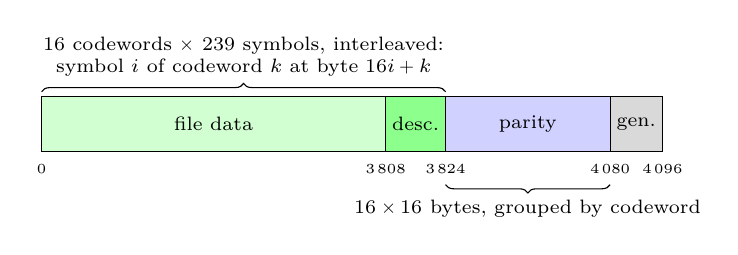
\begin{tikzpicture}[x=0.95mm,y=1mm,font=\scriptsize]
  % not to scale: the coded data is shortened so the small regions read
  \draw[fill=green!18] (0,0) rectangle (46,7);
  \draw[fill=green!45] (46,0) rectangle (54,7);
  \draw[fill=blue!18] (54,0) rectangle (76,7);
  \draw[fill=gray!30] (76,0) rectangle (83,7);
  \node at (23,3.5) {file data};
  \node at (50,3.5) {desc.};
  \node at (65,3.5) {parity};
  \node at (79.5,3.5) {gen.};
  \draw[decorate,decoration={brace,amplitude=3pt}] (0,7.6) -- (54,7.6)
     node[midway,above=2pt,align=center]{16 codewords $\times$ 239 symbols, interleaved:\\symbol $i$ of codeword $k$ at byte $16i+k$};
  \foreach \x/\l in {0/0, 46/3\,808, 54/3\,824, 76/4\,080, 83/4\,096}
     \node[font=\tiny,anchor=north] at (\x,-0.4) {\l};
  \draw[decorate,decoration={brace,amplitude=3pt,mirror}] (54,-4.2) -- (76,-4.2)
     node[midway,below=2pt,align=center]{$16\times16$ bytes, grouped by codeword};
\end{tikzpicture}
\caption{A \bfs data block under \texttt{INCOMPAT\_RS\_INTERLEAVE}, the
layout of every measured volume; byte offsets below, not to scale. The
descriptor (bytes 3\,808 to 3\,823, checksum and self-identifier) is
inside the code and off on the measured volumes; bytes 4\,080 to 4\,095
hold the generation number, outside the code.}
\label{fig:capsule}
\end{figure}

\subsection{Read path}\label{sec:readpath}

Reading a file range, \bfs reads each data block the page overlaps into
a private scratch page, decodes the sixteen codewords there, and copies
the requested bytes out. A 4\,KiB page straddles two 3\,808-byte
payloads, so a sequential read fetches most blocks twice, each time from
the medium. The decoder runs on every read, whatever any checksum says.
If any codeword is beyond correction the read fails with
\texttt{-EIO} and the event is journalled: \bfs refuses rather than
returns bytes it cannot vouch for.

Correction is applied to the copy. In 0.1.26 the read path does not
write the corrected block back. The on-read repair v2 described was
disabled when decoding moved into a private copy; the source states
that re-enabling it needs exclusive access to the block for the whole
read-modify-write. A background scrubber
decodes allocated data blocks at a bounded pace (one block every
100\,ms by default) and writes a corrected block back only if its owner
and its content have not changed in between and the volume is writable.
Errors on the medium are therefore corrected on every read and repaired
by the scrubber, not by the read.

\subsection{Metadata and indirect blocks}\label{sec:indirect-design}

Inodes carry their own RS parity and a CRC over the whole inode;
directory blocks are RS-encoded; the feature bits of every measured
volume read \texttt{incompat}~\featIncompat{} (per-inode RS, indirect
parity, directory RS, full inode CRC, parity-region FEC, interleave) and
\texttt{ro\_compat}~0, which confirms that \texttt{DATA\_CSUM} and
\texttt{DATA\_SELFID} were off.

An indirect block holds 512 raw 64-bit pointers and has no room for its
own code. Its parity lives in a separate region, one slot per indirect
block, by default in Reed-Solomon mode. The slot covers the first 3\,824
bytes, pointers 0 to 477; pointers 478 to 511 are covered by
nothing~\cite{beamfsimpl} (\texttt{known-limitations.md}, 3.38). In
Reed-Solomon mode the verify step decodes a \emph{copy} of the indirect
block, journals what it found and leaves the buffer alone: an earlier
version corrected the live block against stale parity and erased valid
pointers, so a verify no longer writes. A correctable error is thus
journalled and the pointer is read as it stands. Every pointer is then
checked against the data area and the allocation bitmap, and a pointer
outside either fails the lookup with \texttt{-EUCLEAN}. A flipped pointer
that stays inside the data area and lands on an allocated block passes
every check; without \texttt{DATA\_SELFID} nothing detects it. The
project recorded one such case on a direct pointer, 15\,245 wrong bits
returned with no kernel signal (comment in \texttt{file\_inline.c} at
\texttt{\commitBeamfs}). \Cref{sec:indirect} reports what the campaign
did to indirect blocks.

\section{Scope: designed and measured}\label{sec:scope}

The project's data-protection design requires every public artefact to
state its scope in the following normative words, reproduced verbatim
(\texttt{Documentation/data-protection-design.md}, section~7, at
\texttt{\commitBeamfs}; v5.0 names the on-disk format):

\begin{quote}\small
beamfs v5.0 protects against Family A perturbations (stochastic
electromagnetic single-bit and multi-bit upsets, aging silicon bit-rot,
environmental radiation, rowhammer-class single-cell flips). Family B
perturbations (adversarial bursts exceeding 256 octets per sub-block,
IEMI at scale, voltage-glitch attacks at scale) are not claimed by v5.0.
The on-disk format reserves the feature flag bit
\nolinkurl{BEAMFS_FEATURE_INCOMPAT_SHADOW_PARITY} for a future v5.x
revision that adds out-of-band parity with stride placement, targeting
Family B coverage. Coexistence between the two schemes is supported by
design.
\end{quote}

That statement is the design scope. The measured scope of this report is
narrower, and every result below is to be read within it:
\begin{itemize}
\item \emph{one mechanism}: single-bit flips in the data of read bios,
  after the device returned them. The medium is not altered: all
  \flipsAnalysed{} flips recorded on \bfs are on read bios, and after
  every attack, injector off, the twelve files of every filesystem read
  back intact (\cref{sec:multifs});
\item \emph{one load}: at most two flipped bits per read bio, hence at
  most two erroneous symbols per codeword per decode
  (\cref{sec:injector}); multi-bit upsets, bursts and the correction
  limit of eight symbols are not exercised;
\item \emph{one configuration}: on-disk format v5 with interleaving,
  without \texttt{DATA\_CSUM} or \texttt{DATA\_SELFID}, indirect parity
  in Reed-Solomon mode;
\item \emph{one kind of target}: the blocks of one 256\,KiB file
  (its data blocks, plus its indirect block in runs 2 and 3) and,
  through the injector defect of \cref{sec:injector}, the block that
  follows each of them.
\end{itemize}
Nothing here is a physical irradiation, and nothing here measures
Family~B.

\section{Experimental setup}\label{sec:setup}

\paragraph*{Software under test}
\bfs 0.1.26, commit \texttt{\commitBeamfs}, built into one Yocto image
per architecture (layer \texttt{yocto-beamfs} at \texttt{\commitYocto})
with Linux 7.3-rc5 (\texttt{72d3fcf8})~\cite{linux73rc5}, the version
both build configurations pin. \bfs is built into the kernel on both
(\texttt{CONFIG\_BEAMFS\_FS=y}); the module file the images also carry
is never loaded. The two kernels differ in one \bfs option and in their
preemption model. The x86-64 kernel enables
\texttt{CONFIG\_BEAMFS\_DEBUG\_TREE}, which records every pointer stored
in an indirect block, checks each later store to the same slot against
the record, decodes a copy of every parity-region block it has just
encoded, and warns on a violation; these are diagnostics that change
nothing on disk, but cost time and can fail a test through the warning.
The aarch64 kernel does not enable it. The images, the kernels and the
module sources are identified by SHA-256 (\apprepro): every source file
of the module has the same hash in the commit, in the layer, in the run
manifests and in the \srcTrees{} source trees the two builds compiled.
The aarch64 image, \hash{\imageSha}, is checked on every node before each
bench run. The guests boot from \bfs: their root filesystem is a \bfs
volume.

\paragraph*{Machines}
One host (spartian, Gentoo Linux, Intel Core i7-12700F) runs four
aarch64 guests emulated by QEMU without hardware acceleration (machine
\texttt{virt}, Cortex-A57, four vCPUs and 2\,GiB each:
\texttt{beamfs-master}, \texttt{compute01} to \texttt{compute03}) and one
x86-64 guest under KVM (four vCPUs, 8\,GiB). In the cluster campaign each aarch64 node attacks a \bfs
volume on its own virtual disk. The filesystem comparison runs on
\texttt{compute01}, each filesystem on its own USB flash drive,
five drives on the host, each passed to the guest as a virtio block
device.

\paragraph*{Workload}
For each filesystem and each probability, the bench formats the device
(for \bfs, \texttt{mkfs.beamfs -s inline -O per\_inode\_rs}: feature
bits \texttt{incompat}~\featIncompat), writes three directories of three 256\,KiB random files with a SHA-256
list per directory (twelve files), and records the extents of the target
file \texttt{dir-B/file-B2.bin}. An attack reads the target once with the
injector off, as a reference; arms the injector; syncs, unmounts, drops
the caches and mounts again; reads the target and two other files;
disarms the injector. The outcome is decided from the read alone:
\emph{intact} if the bytes read back hash to the recorded value after at
least one flip, \emph{silent corruption} if they do not and the read
succeeded, \emph{read refused} if the read failed, \emph{no flip} if
nothing was injected. A verification then remounts the volume, injector
off, and hashes all twelve files. The cluster campaign runs the same
attack on each node against a file of its \texttt{/data} volume.
The background scrubber of \bfs ran at its default pace throughout.

\paragraph*{Injection}
emufi 0.8.1 (\texttt{srcversion 5DCD6301EB353B0FADD6FE2}) hooks the
block layer with kprobes and flips one bit, at a random position, in the
first segment of a read bio whose sectors match a target filter, with a
probability $p$ per hook invocation; $p$ takes the values $10^{3}$,
$10^{5}$ and $10^{6}$ parts per million. The filter is a list of sector
ranges. emufi refuses a list of more than eight ranges or 512 bytes and
then filters on the interval spanning the file: in runs 2 and 3 the
per-block extent list of \bfs exceeded that limit and the interval,
which includes the file's indirect block, applied; from run 4 the bench
merges contiguous extents and the exact list applied.
\Cref{sec:injector} shows that two hooks act on each \bfs read bio.

\paragraph*{Runs}
Three complete bench runs on the same image, numbered as in the project
log (run 1 stopped before measuring): run 2 (bench
\texttt{\commitBenchTwo}), run 3 (\texttt{\commitBenchThree}) and run 4
(\texttt{\commitBenchFour}). Each writes a GPG-signed manifest of the
chain it measured (\apprepro). Runs 2 and 3 ended with exit
status 1 because some cluster cases were not exercised: in run 2 none,
the injector holding a stale range list from the filesystem comparison;
in run 3 not \texttt{compute01}, whose list emufi refused. Run 4 ended
with status \rcRunFour{}, all twelve cluster cases exercised.

\paragraph*{Functional tests}
xfstests~\cite{fstests} 2024.03.03 as packaged in the images, with three
patches from the layer: \bfs added beside ext2 to the harness's
dispatch on the filesystem type, the volume kept when check declares it
inconsistent, and an upstream fix to generic/589 backported. The
project's harness, beamfs-xfstests~\cite{bx}, runs each test of the
selection in its own invocation of check, on a test volume made by
\texttt{mkfs.beamfs -N 16384}: the \bfs defaults, feature bits
\texttt{incompat}~\featXfstests, the bench's volumes without per-inode
Reed-Solomon. The selection is what check runs when given none, the
\texttt{auto} group: \xfsGenericAuto{} \texttt{generic} and
\xfsSharedAuto{} \texttt{shared} tests, \xfsTotal{} in all, identical on
both images. One sweep per architecture on the same commit, with a
budget of 14\,400\,s per test, aarch64 under harness version 2.3.60 and
x86-64 under 2.5.1, which also records the node, its kernel, its tools,
the features of the volumes it formats, its budget and every recovery
of the node; generic/476 was also run alone on each architecture.

\section{Auditing the injector}\label{sec:injector}

A fault-injection result is only as good as the record of what was
injected. emufi keeps a ring of every flip: sequence number, time,
sector, operation, byte offset in the bio segment, bit, value before and
after. Matching that ring against the corrections the kernel reported
exposed a defect in the record, which this section explains, measures
and works around. emufi is part of the sealed image and was not changed
for this report.

\subsection{Two hooks, one of them a bio early}

emufi 0.8.1 acts on read completions through two kprobes
(\cref{fig:hooks}). The first, on \texttt{blk\_update\_request}, runs
while the bio iterator is intact: it logs the bio's start sector and
flips a bit in its first segment. The block layer then calls
\texttt{bio\_advance} and \texttt{bio\_endio}, where the second kprobe
runs. emufi assumes that by then the iterator has been consumed, the
start sector advanced past the transfer, and recovers the start by
subtracting the transfer size. In Linux 7.3-rc5, \texttt{bio\_advance}
of a complete transfer only zeroes the size and leaves the start sector
where it was (\texttt{include/linux/bio.h} at
\texttt{72d3fcf8}~\cite{linux73rc5}). The second hook therefore logs,
and filters on, the span one bio \emph{before} the bio it flips.

Three consequences follow. A \bfs read bio, one 4\,KiB block, can take
two flips, one per hook, each drawn with probability $p$. The second
flip is logged eight sectors early. And the second hook attacks the
block that follows each target block: in run 4 that put the indirect
block of the target file, which follows its twelfth data block, within
reach although the range list excluded it. A filesystem that reads the
file in multi-block bios is touched by the first hook only, the shifted
span falling before the file: ext4 here, one hook invocation per attack.

\begin{figure}[t]
\centering
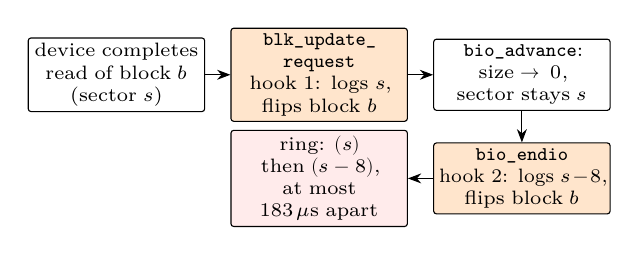
\begin{tikzpicture}[font=\scriptsize,node distance=3.2mm,
  box/.style={draw,rounded corners=1pt,align=center,inner sep=2pt,minimum height=6mm,text width=21mm},
  hook/.style={box,fill=orange!20}]
  \node[box] (dev) {device completes\\read of block $b$\\(sector $s$)};
  \node[hook,right=of dev] (rq) {\texttt{blk\_update\_}\\\texttt{request}\\hook 1: logs $s$,\\flips block $b$};
  \node[box,right=of rq] (adv) {\texttt{bio\_advance}:\\size $\to 0$,\\sector stays $s$};
  \node[hook,below=4mm of adv] (ep) {\texttt{bio\_endio}\\hook 2: logs $s-8$,\\flips block $b$};
  \node[box,left=of ep,fill=red!8] (rec) {ring: $(s)$ then $(s-8)$,\\at most \dtPairMaxMicro\,$\mu$s apart};
  \draw[-{Stealth}] (dev) -- (rq);
  \draw[-{Stealth}] (rq) -- (adv);
  \draw[-{Stealth}] (adv) -- (ep);
  \draw[-{Stealth}] (ep) -- (rec);
\end{tikzpicture}
\caption{The two read hooks of emufi 0.8.1 on Linux 7.3-rc5. Both flip
the block that was read; the second logs it eight sectors (one 4\,KiB
block) early.}
\label{fig:hooks}
\end{figure}

\subsection{Recovering the hook of every flip}

In ring order, an entry at sector $s$ followed within
\dtPairMaxMicro\,$\mu$s by
one at $s-8$ is the pair of one bio, both flips in block $s/8$. At
$p=10^{6}$\,ppm both hooks fire whenever the filter admits them, so an
entry left alone has one explanation: the first hook of a bio whose
shifted span the filter refused (the first target block), or the second
hook of a bio whose own block the filter refused (the block after a
target block). Below $10^{6}$\,ppm either hook may have drawn alone, and
a lone entry is ambiguous between its logged block and the next.

\subsection{Checking the reconstruction}

The reconstruction is checked three ways, all by the extraction script
before any table is written.
\begin{itemize}
\item \emph{Timing.} Over the three $10^{6}$\,ppm attacks, the two
  entries of a pair are at most \dtPairMaxMicro\,$\mu$s apart; two
  consecutive entries that are not a pair are at least
  \dtOtherMinMilli\,ms apart. No interval falls between.
\item \emph{Completeness.} At $10^{6}$\,ppm every flip is attributed
  (\ambiguousHigh{} ambiguous).
\item \emph{The kernel's account.} \bfs logs each correction with the
  inode, the logical block, the codeword and the number of symbols
  corrected, rate-limited to the first ten lines of an attack. All
  \kernLines{} lines are explained by flips at the reconstructed block
  and codeword, or, for an ambiguous flip, at its logged block or the
  next; none is left over. In run 3 at $10^{6}$\,ppm one decode
  corrected two symbols in one codeword: the two flips of one bio, the
  first in that codeword's parity, the second in its data.
\end{itemize}

\Cref{tab:rs} summarises the six \bfs attacks that received flips. With
one bit per hook, a decode sees at most two erroneous symbols in a
codeword; the kernel reported at most \kernMaxPerDecode{}. Taking the
union over a whole attack, which overstates what any decode saw, no
codeword was hit in more than \unionMax{} distinct symbols. The budget
is eight. \Cref{fig:rsmap} shows where the flips fell.

\begin{table*}[t]
\centering
\caption{\bfs attacks with flips: flips received, target filter in
effect, hook pairs and lone entries, kernel lines (all explained), most
symbols corrected in one decode (kernel), most distinct symbols hit in
one codeword over the attack, counting only flips whose block is known
(none at $10^{5}$\,ppm in run 4, where every flip was alone).}
\label{tab:rs}
\footnotesize
\setlength{\tabcolsep}{3pt}
\begin{tabular}{@{}lrrlrrrrr@{}}
\toprule
run & ppm & flips & target & pairs & single & k-lines & dec & union \\
\midrule
2 & 100\,000 & 20 & interval & 2 & 16 & 10 & 1 & 1 \\
2 & 1\,000\,000 & 265 & interval & 132 & 1 & 10 & 1 & 2 \\
3 & 100\,000 & 22 & interval & 1 & 20 & 10 & 1 & 1 \\
3 & 1\,000\,000 & 265 & interval & 132 & 1 & 10 & 2 & 3 \\
4 & 100\,000 & 33 & list & 0 & 33 & 10 & 1 & 0 \\
4 & 1\,000\,000 & 262 & list & 129 & 4 & 10 & 1 & 3 \\
\bottomrule
\end{tabular}

\end{table*}

\begin{figure*}[t]
\centering
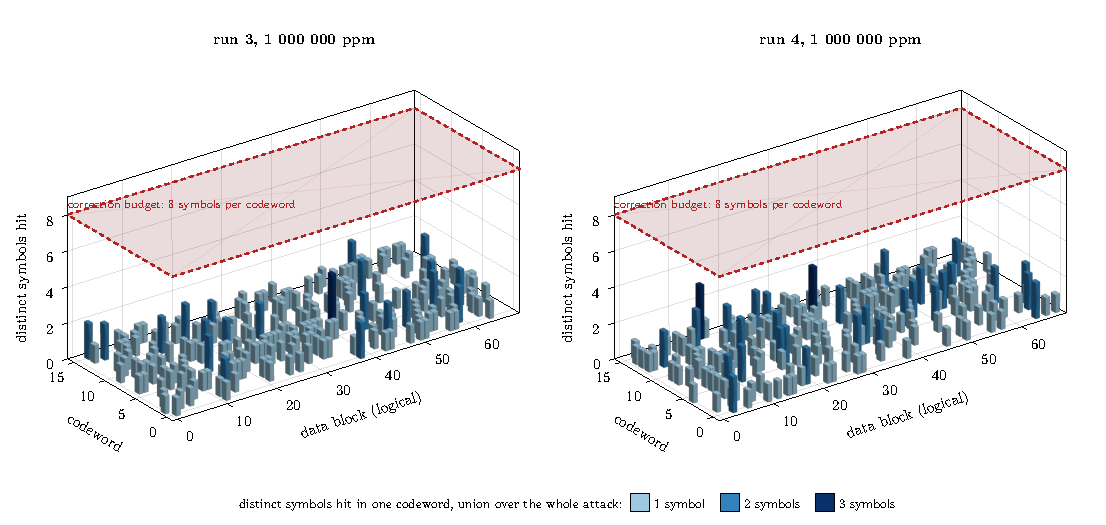
\includegraphics[width=\textwidth]{figures/rsmap-3d.pdf}
\caption{\bfs at $10^{6}$\,ppm, runs 3 and 4: for each data block and
codeword, the number of distinct symbols hit over the whole attack
(flips of known block only). The plane marks the eight symbols one
codeword corrects; no column exceeds \unionMax{}.}
\label{fig:rsmap}
\end{figure*}

\section{Results}\label{sec:results}

\subsection{Functional: xfstests}\label{sec:xfstests}

\Cref{tab:xfs} counts the \xfsTotal{} tests by what check said of each,
read from check's own output for every test. Both sweeps ran on commit
\texttt{\commitBeamfs}, with a budget of 14\,400\,s per test. On x86-64
\xfsXRan{} tests ran and all passed, generic/476, a long multi-process
stress test, in \xfsXfullSeconds\,s. On aarch64 \xfsARan{} ran and
\xfsAPass{} passed; the failure is generic/476, which the harness stopped
at its budget after \xfsAfullSeconds\,s, before check gave a verdict. Run
alone on the same node and image with a longer budget, it passed, in
\xfsAsoloSeconds\,s (\texttt{\sweepAsoloName}).

The other tests did not run: check declined them. On x86-64,
\xfsXNrFeature{} were declined because \bfs does not implement what they
test, \xfsXNrEnv{} because the test image or the virtual machine lacks
what they need, and \xfsXNrScope{} because they apply to other
filesystems only; on aarch64, \xfsANrFeature, \xfsANrEnv{} and
\xfsANrScope. Only \xfsNotrunDifferList{} ran on one architecture and not the
other: it passed on aarch64, and on x86-64 check declined it for want
of procfs \texttt{uid\_map} support. A declined test is untested, not passed: reflinks,
quotas, \texttt{O\_DIRECT}, fallocate modes other than allocation,
encryption, extended attributes and ACLs, among others, are outside what
this suite says about \bfs, and the environment's share (device-mapper
targets, absent tools) is a gap of the test bed, not of \bfs.

These counts are not the ones the harness first printed. Before version
2.4.0 it recorded a declined test as passed, because check counts it in
its ``Passed all'' line, and the aarch64 sweep was saved as 733 passes
and one failure. The aarch64 counts here are recomputed from the output
of check that the harness kept for each test; the x86-64 sweep was run
again under 2.5.1, which records a declined test as such, its budget and
every recovery of the node (\cref{sec:selfaudit}). Two earlier x86-64
sweeps of the same commit are superseded: one saved as 734 passes, whose
per-test output was overwritten by the sweeps that followed, and one
stopped after \xfsSupDone{} tests once its budget, the default
1\,900\,s, had stopped generic/476.

\begin{table}[t]
\centering
\caption{xfstests auto group, \xfsTotal{} tests, by what check said of
each test. Declined tests by the reason check gave; groups of fewer
than four tests are summed per kind, all \xfsGroups{} are in the
derived file xfstests.csv.}
\label{tab:xfs}
\footnotesize
\begin{tabular}{@{}llrr@{}}
\toprule
 & & x86-64 & aarch64 \\
\midrule
passed & & 122 & 122 \\
failed & & 0 & 1 \\
declined by check & & 612 & 611 \\
\midrule
\multicolumn{4}{@{}l}{declined for} \\
\quad reflink & feature & 172 & 172 \\
\quad fallocate modes & feature & 66 & 66 \\
\quad O\_DIRECT & feature & 50 & 50 \\
\quad quotas & feature & 30 & 30 \\
\quad shutdown ioctl & feature & 29 & 29 \\
\quad encryption & feature & 26 & 26 \\
\quad extended attributes & feature & 22 & 22 \\
\quad exchange-range & feature & 19 & 19 \\
\quad deduplication & feature & 14 & 14 \\
\quad ACLs & feature & 13 & 13 \\
\quad inode flags & feature & 12 & 12 \\
\quad swap files & feature & 12 & 12 \\
\quad device nodes, FIFOs & feature & 8 & 8 \\
\quad idmapped mounts & feature & 6 & 6 \\
\quad freeze & feature & 5 & 5 \\
\quad O\_TMPFILE & feature & 4 & 4 \\
\quad renameat2 flags & feature & 4 & 4 \\
\quad 13 other features & feature & 19 & 19 \\
\addlinespace[2pt]
\quad device-mapper target & environment & 48 & 48 \\
\quad tool absent from the image & environment & 16 & 16 \\
\quad richacl & environment & 9 & 9 \\
\quad device size & environment & 7 & 7 \\
\quad DAX & environment & 5 & 5 \\
\quad log device & environment & 4 & 4 \\
\quad scsi\_debug & environment & 4 & 4 \\
\quad 4 other needs & environment & 5 & 4 \\
\addlinespace[2pt]
\quad other filesystems only & scope & 3 & 3 \\
\bottomrule
\end{tabular}

\end{table}

\subsection{Filesystem comparison}\label{sec:multifs}

\Cref{fig:multifs} shows run 4 and \cref{tab:multifs} all three runs.
\bfs returned the correct file in every attack that received flips, up
to \mfBeamfsMaxFlips{} flips during one read, in all three runs. At
$10^{6}$\,ppm, ext4 returned wrong data with a successful read after
\mfExtFourFlipsMax{} flip, ext3 after \mfExtThreeFlipsMin{} to
\mfExtThreeFlipsMax{}, in every run: silent corruption. btrfs, after
\mfBtrfsFlipsMin{} flips, refused the read on a checksum mismatch.
squashfs was never exercised: the bench builds its image offline and
gave the injector no target.

The doses differ by design and are reported as received, not equalised.
emufi draws once per hook and per bio, and a filesystem receives flips
in proportion to the bios its read issues: one for ext4, about two per
data block for \bfs (\cref{sec:readpath}), which is why the other
filesystems received no flip at $10^{3}$ and $10^{5}$\,ppm. What the
comparison measures is the outcome per flip received: \bfs absorbed two
orders of magnitude more flips than any other filesystem and returned
the right bytes; ext4 and ext3 returned wrong bytes without an error;
btrfs detected and refused. It is not a ranking of these filesystems in
general.

After every attack the volume was remounted with the injector off and
all twelve files of every filesystem hashed intact, including those of
ext4 and ext3 after their silent corruption: the wrong bytes were made
in the read path, not on the medium.

\begin{figure}[t]
\centering
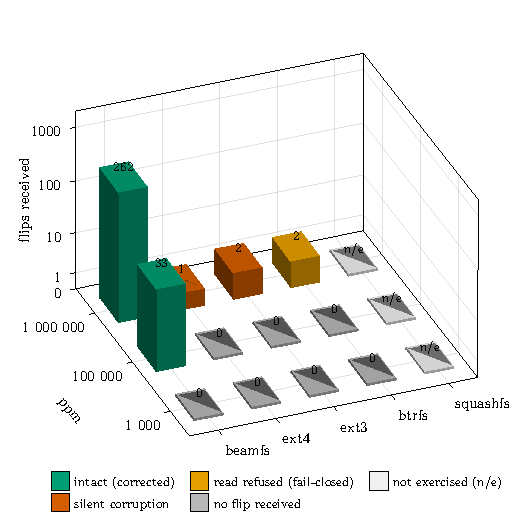
\includegraphics[width=\columnwidth]{figures/multifs-3d.pdf}
\caption{Filesystem comparison, run 4: flips received during one read
of the target file (logarithmic, number on each bar) and outcome, for
each injection probability per hook call (ppm).}
\label{fig:multifs}
\end{figure}

\begin{table}[t]
\centering
\caption{Filesystem comparison, three runs: flips received and outcome
(I intact, S silent corruption, R read refused, N no flip,
n/e not exercised).}
\label{tab:multifs}
\footnotesize
\begin{tabular}{@{}llccc@{}}
\toprule
FS & ppm & run 2 & run 3 & run 4 \\
\midrule
beamfs & 1\,000 & 0\,N & 0\,N & 0\,N \\
 & 100\,000 & 20\,I & 22\,I & 33\,I \\
 & 1\,000\,000 & 265\,I & 265\,I & 262\,I \\
\addlinespace[2pt]
ext4 & 1\,000 & 0\,N & 0\,N & 0\,N \\
 & 100\,000 & 0\,N & 0\,N & 0\,N \\
 & 1\,000\,000 & 1\,S & 1\,S & 1\,S \\
\addlinespace[2pt]
ext3 & 1\,000 & 0\,N & 0\,N & 0\,N \\
 & 100\,000 & 0\,N & 0\,N & 0\,N \\
 & 1\,000\,000 & 3\,S & 2\,S & 2\,S \\
\addlinespace[2pt]
btrfs & 1\,000 & 0\,N & 0\,N & 0\,N \\
 & 100\,000 & 0\,N & 0\,N & 0\,N \\
 & 1\,000\,000 & 2\,R & 2\,R & 2\,R \\
\addlinespace[2pt]
squashfs & 1\,000 & n/e & n/e & n/e \\
 & 100\,000 & n/e & n/e & n/e \\
 & 1\,000\,000 & n/e & n/e & n/e \\
\bottomrule
\end{tabular}

\end{table}

\subsection{Cluster}\label{sec:cluster}

In run 4 all twelve cases were exercised (\cref{fig:cluster},
\cref{tab:cluster}): \clRunFourIntact{} returned the correct file after
flips, \clRunFourNoFlip{} received none at $10^{3}$\,ppm. In run 3,
\texttt{compute01} was not exercised, and \texttt{beamfs-master} at
$10^{6}$\,ppm refused the read after \clRunThreeRefusedFlips{} flips
(\cref{sec:indirect}). In run 2 no cluster case was exercised.

\begin{figure*}[t]
\centering
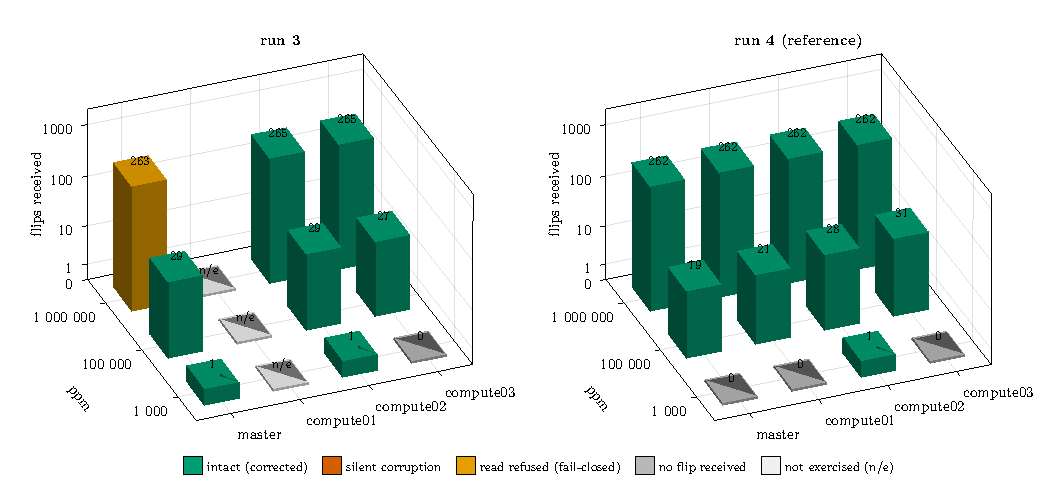
\includegraphics[width=\textwidth]{figures/cluster-3d.pdf}
\caption{Cluster campaign, runs 3 and 4: flips received by each node's
attack and outcome, for each injection probability per hook call (ppm).}
\label{fig:cluster}
\end{figure*}

\begin{table}[t]
\centering
\caption{Cluster campaign: flips received and outcome (codes as in
\cref{tab:multifs}). Run 2 exercised no case.}
\label{tab:cluster}
\footnotesize
\begin{tabular}{@{}llcc@{}}
\toprule
node & ppm & run 3 & run 4 \\
\midrule
master & 1\,000 & 1\,I & 0\,N \\
 & 100\,000 & 29\,I & 19\,I \\
 & 1\,000\,000 & 263\,R & 262\,I \\
\addlinespace[2pt]
compute01 & 1\,000 & n/e & 0\,N \\
 & 100\,000 & n/e & 21\,I \\
 & 1\,000\,000 & n/e & 262\,I \\
\addlinespace[2pt]
compute02 & 1\,000 & 1\,I & 1\,I \\
 & 100\,000 & 29\,I & 28\,I \\
 & 1\,000\,000 & 265\,I & 262\,I \\
\addlinespace[2pt]
compute03 & 1\,000 & 0\,N & 0\,N \\
 & 100\,000 & 27\,I & 31\,I \\
 & 1\,000\,000 & 265\,I & 262\,I \\
\bottomrule
\end{tabular}

\end{table}

\subsection{Indirect blocks}\label{sec:indirect}

In run 3 the cluster filter was the interval spanning the file, which
contains its indirect block. On \texttt{beamfs-master} at
$10^{6}$\,ppm the kernel logged four times
\begin{lstlisting}
beamfs/inline: corrupted indirect pointer ino=11 iblock=45
  slot=33 phys=18014398509500044 (out of [17502, 262144))
\end{lstlisting}
\noindent That value is
$2^{54}+18\,060$: bit 54 of the pointer in slot 33 was flipped in the
read buffer, the true pointer being 18\,060. On this code path the
Reed-Solomon verify decodes a copy of the freshly read indirect block,
finds a correctable error and lets the lookup proceed
(\cref{sec:indirect-design}); the lookup read the pointer from the
buffer, found it outside the data area and failed. The read was refused,
no wrong byte was returned, and the twelve files verified intact
afterwards.

In the filesystem comparison the reconstruction of
\cref{sec:injector} attributes \indHits{} flips to the target file's
indirect block, at slots \indSlots{}, including one in run 4 through the
second hook. The file uses 57 pointers (69 data blocks, 12 of them
direct), slots 0 to 56: none of these flips touched a pointer in use,
and the reads were unaffected.

These events show the fail-closed contract holding for a pointer flipped
out of range. They do not test the residual of
\cref{sec:indirect-design}: a flip that keeps a pointer inside the data
area and on an allocated block would, on these volumes, return another
block's bytes.

\section{A parallel with proton irradiation}\label{sec:memon}

Memon et al.~\cite{memon2025tr,memon2025arxiv} exposed three commercial
compute modules running Linux to 20 to 58\,MeV protons at the AIC-144
cyclotron of IFJ PAN, Krak\'ow: a Raspberry Pi Zero~2~W, an NXP
i.MX~8M~Plus board (Yocto Linux 5.15.77, root filesystem ext4 on eMMC)
and an OrangeCrab FPGA board running a VexRiscv soft core. They record
133 Linux single-event functional interrupts across the three, and on
the i.MX~8M~Plus attribute 56\,\% of failures to the filesystem and
34\,\% to the storage driver, up to ext4 journal aborts and read-only
remounts~\cite{memon2025arxiv}. The work follows failures of unmodified
Linux on commercial modules down to the kernel subsystem, across three
architectures, with failure cross-sections per platform and energy. That
resolution is what makes it usable by a filesystem designer, and its
finding that the storage path dominates on the i.MX~8M~Plus is the
observation \bfs answers. Their result and ours meet at the storage
path; \cref{tab:memon} sets the two methods side by side.

\begin{table}[t]
\centering
\caption{Physical irradiation~\cite{memon2025arxiv} and this report.}
\label{tab:memon}
\footnotesize
\begin{tabularx}{\columnwidth}{@{}>{\raggedright\arraybackslash}p{1.3cm}
  >{\raggedright\arraybackslash}X >{\raggedright\arraybackslash}X@{}}
\toprule
 & Memon et al. & this report \\
\midrule
cause & protons, 20 to 58\,MeV & emulated single-bit flips \\
where & SoC die (and memory, see text) & read-bio buffers of chosen blocks \\
effects & any: crashes, hangs, driver and filesystem errors &
  wrong bytes delivered to the filesystem only \\
filesystem & ext4 on eMMC & \bfs, ext4, ext3, btrfs, squashfs \\
observable & failure class per run & outcome per read; kernel
  corrections per decode \\
dose & fluence per run & flips received per attack \\
hardware & exposed; replaced by an unexposed unit after each fluence;
  not reported retested & not exposed; medium verified unaltered after
  every attack \\
\bottomrule
\end{tabularx}
\end{table}

The two are complementary. A beam reproduces physics no emulator does:
controller hangs, crashes, the faults their failure classes record. It
is costly, and each unit absorbs dose. Emulation injects one mechanism,
at chosen blocks, with a record of every flip, and leaves the hardware
untouched; it cannot say what a beam does to a controller. \bfs
addresses only the bytes a read returns: against a hung eMMC controller
it can at best fail closed.

\subsection{What a failure class says about the hardware}

A beam acts on hardware; software only reports what follows. Telling
the two apart is what lets a failure be read as a single-event effect on
a sound device rather than as the symptom of a damaged one, so we read
both texts on that point.

Their protocol is careful about cumulative damage. Failures are observed
through software-visible channels, the kernel log, the system journal
and user-space signals, logged off the device, and root causes are
attributed by kernel log forensics; each run ends at its first
functional interrupt~\cite{memon2025arxiv}. Supply current and voltage
are logged throughout. After each targeted fluence every device is
replaced by an identical, previously unexposed copy, so that total
ionising dose and displacement damage do not bias the
analysis~\cite{memon2025arxiv}; the journal manuscript replaces devices
after each test objective and mentions real-time detection of current
latch-ups~\cite{memon2025tr}, while the arXiv text places single-event
latch-up, micro-latch-up included, outside its scope. For one memory
error the authors note that a prior clean run weakens the hypothesis of
a permanent cell defect~\cite{memon2025arxiv}.

What a failure class cannot say is what the beam did to the hardware. On
the i.MX~8M~Plus a filesystem error has at least three physical
readings, which the logs alone do not separate:
\begin{enumerate}[label=(\roman*)]
\item a transient upset in the system on chip, in a core, a cache, the
  storage host controller or a DMA engine, that corrupts data or kernel
  state in flight and leaves the hardware intact;
\item data altered on the eMMC itself, by an upset in the eMMC if it was
  in the beam, or by the system on chip writing corrupted data, which
  survives a power cycle;
\item a part degraded by its dose, through ionising dose, displacement
  damage or a micro-latch-up, that no longer behaves as a fresh one.
\end{enumerate}
They call for different remedies, and only the first is a property of
software running on sound hardware; the second and third are effects on
hardware that software then reports. The checks that separate them are a readback of the storage
against its pre-exposure image, a functional and electrical test of each
unit after its exposure (supply current at rest against its pre-exposure
value, a memory test), and the dose each unit received. Neither text
reports them, and neither states where the units came from. Replacing
units between fluences keeps damage from carrying into the next run; it
does not show that a unit was intact at the end of its own run, and a
cross-section computed over all the runs at one energy assumes every
unit equivalent and unaltered throughout. The modules are commercial parts, not hardened
ones, and their own tolerance is precisely what is left unmeasured: the
campaign establishes how often these systems fail under protons, not how
much the hardware itself withstands, nor, for a given failure, whether
software met a transient upset or a damaged device.

The beam geometry on the i.MX~8M~Plus is also stated three ways: the
journal manuscript puts the system on chip and the LPDDR4 memory in the
beam; the arXiv text puts only the system-on-chip die in the beam
aperture, external memory and storage outside; its Table~1 lists the
system on chip, the LPDDR4 and the eMMC as irradiated. Whether the eMMC
and the memory were exposed changes which readings are possible for
90\,\% of that board's failures.

This matters to \bfs directly. It covers reading (i) when the upset
corrupts the bytes a read returns, and reading (ii) when the altered
bytes stay within its correction capacity; it can do nothing for
corrupted kernel state or a degraded controller, where it can at best
fail closed. Which reading dominates is therefore the first question a
beam campaign on \bfs must answer, and the one this emulation sidesteps
by construction: here the hardware is not exposed, and the medium was
read back intact after every attack (\cref{sec:multifs}).

These are reporting points, not evidence against the measurements, which
we take as they are reported. A beam campaign on \bfs would need them
settled from the start: unit provenance and pre-exposure
characterisation, dose per unit, a post-exposure functional and
electrical test of every unit, a readback of the storage against its
pre-exposure image, and the exact parts in the beam.

\subsection{The same questions, asked of this report}\label{sec:selfaudit}

The checks we ask of a beam campaign apply to this report too, with the
instruments in the place of the hardware. Each item says what was
checked and what was found.

\begin{enumerate}[label=(\alph*)]
\item \emph{What was measured.} The units here are software, named by
  their hashes: the \bfs commit, the Yocto layer, the root image and the
  kernel of each architecture, and \srcTrees{} compiled source trees found
  identical to the sources the signed manifests list (\apprepro). \bfs
  is built into both kernels; the module file its recipe also installs
  is never loaded. The tools are identified by SHA-256 against the
  repository, not by the version they print (mkfs.beamfs prints
  \xfsXMkfsVersion, fsck.beamfs \xfsXFsckVersion, the module is 0.1.26).
  The two kernels differ in one \bfs option: the x86-64 kernel has
  the tree checker \texttt{CONFIG\_BEAMFS\_DEBUG\_TREE}
  (\cref{sec:setup}); the aarch64 kernel, on which every attack ran, does
  not. The x86-64 xfstests sweep ran with more internal checks than the
  attacks.
\item \emph{State after exposure.} The attacks leave the medium
  untouched by construction, and it was read back after every attack:
  twelve files intact on every filesystem (\cref{sec:multifs}). For the
  x86-64 sweep, the node ran without a restart: the harness recorded no
  recovery, and the node's uptime grew by the length of the sweep. Its
  kernel taint flags read \xfsXtaintStart{} at the start and the same at
  the end, without the warning or the oops flag: no kernel warning and
  no oops occurred. The harness clears the kernel log before each test
  and keeps it after; none of the \xfsXkernLogs{} logs holds a warning or
  an oops, and in \xfsXtreeLogs{} of them the tree checker reported no
  lost pointer.
\item \emph{Dose.} Every flip is in the injector's ring and is matched
  against the kernel's own record of each correction
  (\cref{sec:injector}); doses still differ between filesystems
  (\cref{sec:limits}).
\item \emph{What the instruments reported.} Our own tools misreported,
  and each defect was found by reading a raw record against an
  independent account of the same event.
  \begin{itemize}
  \item emufi logs a hook one bio early on this kernel, found against
    the kernel's correction lines (\cref{sec:injector}).
  \item The xfstests harness, before 2.4.0, saved a test that xfstests
    declined as passed, because check counts it in its ``Passed all''
    line; found against check's own output for each test. Before 2.3.61
    the per-test output of a sweep was overwritten by the next one. 2.4.0
    asked the node for a module source version that \bfs does not
    expose, and recorded an empty field. All three are corrected in
    2.5.0, and the x86-64 sweep was run again under 2.5.1; the counts of
    \cref{tab:xfs} are read from check's output, not from the harness's
    summary.
  \item The first x86-64 sweep under 2.5.0 ran under the harness's
    default budget of 1\,900\,s per test, below the \xfsXsoloSeconds\,s
    generic/476 had taken alone on the same image, and the budget, not
    \bfs, stopped the test after \xfsSupFullSeconds\,s. That budget was
    ours to set, and the record did not name it. The sweep was stopped
    after \xfsSupDone{} tests; the harness now records its budget and
    every recovery of the node (2.5.1), and the sweep was run again
    under 14\,400\,s, in which generic/476 passed.
  \item The bench's record of each btrfs attack has no checksum line in
    its slice of the kernel log; the cause of the refusal, a
    \texttt{csum failed} warning on mirror~1, is read from the node's
    own kernel log, where it appears in each run. The bench's topology
    report calls \bfs a loaded module while it is built in. Correction
    lines are rate-limited (\cref{sec:limits}).
  \end{itemize}
\item \emph{What the tools did not reach.} squashfs was never attacked:
  its attack printed no target in any run. The write path received
  no flip. xfstests declined \xfsXNotrun{} tests on x86-64 and
  \xfsANotrun{} on aarch64 (\cref{sec:xfstests}); they are untested.
\end{enumerate}

Two of these defects would have changed a result had the raw records
not been read: which block each flip hit, and the xfstests counts; a
third, the budget, would have reported generic/476 as failed on x86-64.
The
others change no number in this report; they are listed so that they
are corrected before the next campaign. All are in the tools; none is
in the \bfs code measured here.

\section{What beamfs brings}\label{sec:brings}

The measurements answer a narrow question. This section places the
answer among the ways a system can get the right bytes back after a bit
flips between the medium and the filesystem.

\begin{table}[t]
\centering
\caption{Getting correct data back after a flipped bit in file data.
``Measured'' means measured in this report; other rows are as
documented.}
\label{tab:position}
\footnotesize
\begin{tabularx}{\columnwidth}{@{}>{\raggedright\arraybackslash}p{2.0cm}
  >{\raggedright\arraybackslash}X >{\raggedright\arraybackslash}p{1.45cm}@{}}
\toprule
filesystem & on a flipped bit in file data & extra space \\
\midrule
ext4, ext3 & wrong bytes returned, no error (measured) & none \\
btrfs, data \texttt{single} & detected, read refused (measured) &
  checksums \\
btrfs, data \texttt{DUP} or RAID1 & detected, served and repaired from
  the other copy~\cite{btrfsautorepair} & a full copy \\
ZFS, \texttt{copies=2} & detected, repaired from the other
  copy~\cite{zfschecksums} & a full copy~\cite{zfsprops} \\
\bfs capsule & corrected on read up to 8 symbols per codeword, measured
  up to \kernMaxPerDecode{}; refused when the decoder fails; beyond 8, a
  wrong decode is possible without \texttt{DATA\_CSUM} & 288 bytes
  per 4\,096 (7.0\,\%) \\
\bottomrule
\end{tabularx}
\end{table}

\paragraph*{The contribution}
\bfs corrects file data inside the filesystem, on one medium, for 288
bytes in 4\,096: 256 of parity, 16 of descriptor, 16 of generation.
Redundancy also returns correct data (\cref{tab:position}), at the price
of a second copy of every block, and for RAID1 of a second device. The
two protect against different damage: a second copy survives anything
that spares it, a capsule only damage within its correction capacity.
They combine, since a \bfs volume can sit on a mirror. Where a second
copy does not fit, on a single small medium in an embedded, edge or
space system, correction inside the filesystem is what remains; that is
the case \bfs is built for. This report argues that case from the
design, not from a measurement against redundancy, which is planned
(\cref{sec:v4}).

Around that core, \bfs brings: correction on every read, not only once a
checksum has failed; an error instead of bytes the decoder could not
vouch for; a 64-entry correction journal in the superblock recording
block, codeword and symbols corrected; a scrubber that decodes blocks no
one reads and writes corrected ones back; interleaving, so that a burst
in the coded bytes is spread over sixteen codewords
(\cref{sec:capsule}). And it comes with a measurement chain others can
repeat: signed manifests, frozen snapshots, and an audit that found a
defect in its own injector (\cref{sec:injector}).

\paragraph*{What it costs}
288 bytes in 4\,096 of capacity. A Reed-Solomon encode on every write:
v2 measured a median write-and-fsync latency 7.84 times that of ext4
(2.73 times at the 99th percentile), under emulation and on an earlier
layout~\cite{desbrieres2026beamfsv2}; the write path has changed since
and v3 measures no performance. A sequential read fetches most blocks
twice (\cref{sec:readpath}). \moduleLines{} lines of code outside the
kernel tree, with buffer heads still under the metadata.

\paragraph*{Where it is not better today}
Pointers: in the default configuration a flipped indirect pointer that
stays in range is not detected (\cref{sec:indirect-design}), where ext4
with \texttt{metadata\_csum} checksums every extent block~\cite{ext4csum}
and btrfs checksums data and metadata by default~\cite{btrfscsum}.
Inodes: one codeword each, so nine consecutive bytes lose the inode and
the file with it, which interleaving cannot help
(\texttt{burst-resistance.md}). Parity: grouped per codeword, so nine
bytes suffice there too (\cref{sec:capsule}). And the project's own
notes say the default indirect-parity mode should not ship as default
until indirect blocks carry a generation (\cref{sec:limits}, item~\ref{lim:indirect}).

\section{Limitations}\label{sec:limits}

Each item narrows what the results support.

\begin{enumerate}
\item \emph{Emulation, not physics.} Every upset is a bit flipped in a
  read buffer by software. Nothing here is a radiation measurement, and
  no result transfers to a beam without one.
\item \emph{The correction limit is not exercised.} At most two
  erroneous symbols reached a codeword in one decode, against eight
  correctable. Multi-bit upsets, bursts, and the regime beyond eight
  symbols, where a Reed-Solomon decoder can miscorrect silently
  (\texttt{known-limitations.md}, 3.11), are untested. The measured
  volumes did not carry \texttt{DATA\_CSUM}, which exists to catch
  that case.
\item \emph{Grouped parity.} Nine consecutive bytes in the parity of one
  codeword defeat it (\cref{sec:capsule}); burst tolerance holds for the
  3\,824 coded bytes only.
\item\label{lim:indirect} \emph{Indirect blocks.} In Reed-Solomon mode the indirect parity
  detects and journals but does not repair the buffer; pointers 478 to
  511 have no parity; a pointer flipped within the data area onto an
  allocated block is not detected without \texttt{DATA\_SELFID}
  (\cref{sec:indirect-design}). The project's own notes advise against
  Reed-Solomon as the default indirect-parity mode until a per-block
  generation covers indirect blocks (\texttt{known-limitations.md},
  3.13).
\item \emph{The instrument.} emufi 0.8.1 logs one hook a bio early on
  this kernel (\cref{sec:injector}). Below $10^{6}$\,ppm a lone flip's
  block is known only to within one block. The effective target
  included the block after each target block. emufi seeds its generator
  at load, so an attack is reproducible in its parameters, not bit for
  bit.
\item \emph{Unequal doses.} Flips follow bios, and filesystems issue
  different numbers of bios for the same read. Results are reported per
  flip received, not at equal exposure.
\item \emph{Coverage of the campaign.} Three runs; one target file per
  attack; static workload. squashfs was never exercised. In runs 2 and 3
  part of the cluster was not exercised (\cref{sec:setup}).
\item \emph{Functional coverage.} xfstests ran its \texttt{auto} group
  and declined \xfsXNotrun{} of its \xfsTotal{} tests on x86-64 and
  \xfsANotrun{} on aarch64 (\cref{tab:xfs}); what they test is untested
  here. The tree checker of the x86-64 kernel was not built into the
  aarch64 kernel (\cref{sec:setup}).
\item \emph{generic/476 on aarch64.} Within the sweep the harness
  stopped it at its time budget while it was still writing. Its reading
  of the volume images taken then, mounted and in use, found block
  pointers beyond the end of the device; an image of a volume in use
  cannot tell damage on disk from writes in flight, and the question is
  left open. Run alone on the same image the test passed, and it passed
  in the x86-64 sweep.
\item \emph{Tool reporting.} The bench and the xfstests harness
  misreported in ways listed in \cref{sec:selfaudit}; the results here
  are read from the raw records, not from their summaries.
\item \emph{Kernel log.} Correction lines are rate-limited: the
  per-decode figures rest on the first ten lines of each attack.
\item \emph{Platform.} Virtual machines on one host; virtual disks and
  USB flash media with their own controllers and error correction
  below the filesystem. Nothing was run on target hardware.
\item \emph{Write path.} emufi's write hook was armed but recorded no
  flip on \bfs; upsets on the write side are untested.
\item \emph{Size.} At \moduleLines{} lines the module is beyond the
  5\,000-line audit budget the project once set itself.
\end{enumerate}

\section{Toward v4}\label{sec:v4}

The next report has two jobs: close what this one found open, and
measure what this one could not. Each item names its source, a project
document at \texttt{\commitBeamfs} or a finding of this report.

\paragraph*{Format and code}
\begin{enumerate}
\item \emph{Indirect blocks, whole and dated.} A parity slot of 18
  codewords, 288 bytes, covering all 4\,096 bytes of the block behind a
  new incompatible feature bit (\texttt{format-v6.md}, section~8); and a
  per-block generation, so that a verify can tell stale parity from
  damage and repair the block instead of only journalling the error
  (\texttt{known-limitations.md}, 3.13). Until then, the CRC mode of
  indirect parity refuses a block that fails its check, where the
  Reed-Solomon mode journals a correctable error and serves the block as
  read (\texttt{indparity.c}).
\item \emph{\texttt{DATA\_CSUM} and \texttt{DATA\_SELFID} by default.}
  The first catches a codeword decoded wrongly beyond eight errors
  (\texttt{known-limitations.md}, 3.11); the second, a pointer that
  reaches the wrong data block (\texttt{capsule.md}). Both exist, behind
  \texttt{mkfs.beamfs --data-csum}, and were off on every measured
  volume.
\item \emph{Parity interleaving}, from this report: spread the parity
  symbols as the data symbols are, so that nine bytes no longer suffice
  anywhere in the block, and measure the cost. Reconcile the 129-byte
  burst the geometry gives (\cref{sec:capsule}) with the 139 bytes
  recorded from the kernel's codec (\texttt{capsule.md}).
\item \emph{Inode replicas}, studied but not decided
  (\texttt{burst-resistance.md}): the one structure interleaving cannot
  protect.
\item \emph{Read path}, from this report: stop fetching each block twice
  on a sequential read, and restore on-read repair with exclusive access
  to the block or by copy-on-write.
\item \emph{Family~B}: the reserved \texttt{SHADOW\_PARITY} feature,
  out-of-band parity placed by stride, is the format's path toward the
  perturbations the scope of \cref{sec:scope} does not claim
  (\texttt{data-protection-design.md}, \texttt{format-v5.md}).
\item \emph{Security review}: stage~5 of the project roadmap, syzkaller
  on the module's system-call surface, afl++ on \texttt{mkfs.beamfs}
  and on mount-time parsing of corrupted images, a fault-injection
  harness, and an adversarial review against Family~B
  (\texttt{roadmap.md}).
\end{enumerate}

\paragraph*{Measurement}
\begin{enumerate}
\item \emph{Fix the injector} (\cref{sec:injector}), then inject what v3
  did not: multi-bit upsets and bursts up to and beyond eight symbols
  per codeword, with \texttt{DATA\_CSUM} on; flips on the write path;
  in-range pointer flips on indirect blocks.
\item \emph{Equal doses}: a fixed number of flips per filesystem rather
  than a probability per bio.
\item \emph{The right reference points}: btrfs with \texttt{DUP} data
  and ZFS with \texttt{copies=2}, which also return correct data, at
  their space cost.
\item \emph{Performance} on target hardware, against ext4 and btrfs.
\item \emph{The instruments' own records}, from this report: the defects
  of \cref{sec:selfaudit} corrected in the bench, the kernel's \bfs
  options recorded by the xfstests harness, the tests the environment
  declined given what they need, a budget per test set from its known
  duration, and the frozen aarch64 volume of generic/476 explained.
\item \emph{A beam campaign} with the hardware record of
  \cref{sec:memon}: unit provenance and pre-exposure characterisation,
  dose per unit, a post-exposure test of every unit, a readback of the
  storage against its pre-exposure image, and the exact parts in the
  beam.
\end{enumerate}

\section{Conclusion}\label{sec:conclusion}

\bfs 0.1.26 passed all \xfsXRan{} xfstests tests that ran on x86-64
and \xfsAPass{} of the \xfsARan{} that ran on aarch64, out of
\xfsTotal{}; xfstests declined the others, which are untested. Under
emulated single-bit upsets on the read path, it never returned wrong
data: it returned the correct bytes after every
flip that reached a data block and refused the one read it could not
vouch for. In the same
conditions ext4 and ext3 returned wrong data without an error and btrfs
refused. These results are bounded by their load, at most
\kernMaxPerDecode{} erroneous symbols per codeword and per decode against
eight correctable; the correction limit, bursts and miscorrection remain
to be measured, with \texttt{DATA\_CSUM} enabled.

Two findings matter beyond the numbers. The injector's record was wrong
in a way the outcomes alone would never have shown; checking it against
the kernel's own account of each correction found the error, and its
cause in the kernel source. And the indirect-block parity, as built,
detects without repairing, which leaves a pointer flipped onto another
allocated block undetected on volumes without \texttt{DATA\_SELFID}.
Both are stated here so that the next measurement, on a beam or on a
corrected injector, starts from them.

Is \bfs worth having? Where a second copy of the data fits, redundancy
already returns correct data and \bfs is at most a complement to it.
Where it does not, on one small medium, \bfs returned correct data or,
once, refused, for 7\,\% of capacity, where ext4 and ext3 returned wrong
data and btrfs could only refuse (\cref{sec:brings}). That is a narrow claim,
bounded by the load measured here, and v4 is planned to widen it or to
find where it stops (\cref{sec:v4}).

\section*{Disclosure}
The analysis scripts and the draft of this report were written with the
assistance of Claude Opus 5.5 (model \texttt{claude-opus-5-5}, Anthropic). Every
measurement was taken by the author's tooling on the author's machines,
and every number in the text is generated from the run records as
described in \apprepro.


\printbibliography

\onecolumn
\small
\section*{Appendix: reproducibility and claims register}
\phantomsection\label{sec:repro}
\addcontentsline{toc}{section}{Appendix: reproducibility and claims register}

\paragraph*{Measured chain}
\bfs commit \hash{\commitBeamfsFull}; Yocto layer \texttt{\commitYocto};
Linux 7.3-rc5, commit \texttt{72d3fcf802c45d00b300f25b848a93c3a2bd7c7e};
root images SHA-256: x86-64 \hash{\imageXSha}, aarch64 \hash{\imageSha};
kernels SHA-256: x86-64 \texttt{bzImage} \hash{\kernelXSha}, aarch64
\texttt{Image} \hash{\kernelASha}; \bfs built in on both
(\texttt{CONFIG\_BEAMFS\_FS=y}), \texttt{CONFIG\_BEAMFS\_DEBUG\_TREE=y}
on x86-64 only; \srcTrees{} compiled source trees identical to the
sources the manifests list; on x86-01, mkfs.beamfs \hash{\xfsXMkfsSha}
and fsck.beamfs \hash{\xfsXFsckSha}; emufi 0.8.1,
\texttt{srcversion 5DCD6301EB353B0FADD6FE2}; bench commits
\texttt{\commitBenchTwo}, \texttt{\commitBenchThree},
\texttt{\commitBenchFour} for runs 2, 3, 4.

\paragraph*{Signed manifests}
Each run manifest is signed with the author's key
\texttt{319A 8EAA 89C7 538A A955 0E8B C35E E212 519E 4857} (EdDSA) and
verified before extraction.
\begin{itemize}
\item run 2, \texttt{\manifestNameTwo}: \hash{\manifestShaTwo}
\item run 3, \texttt{\manifestNameThree}: \hash{\manifestShaThree}
\item run 4, \texttt{\manifestNameFour}: \hash{\manifestShaFour}
\end{itemize}

\paragraph*{xfstests records}
\begin{itemize}
\item x86-64 sweep, harness 2.5.1, \texttt{\xfsXtag}: \texttt{meta.txt}
  \hash{\xfsXmetaSha}, \texttt{verdicts.txt} \hash{\xfsXverdictsSha},
  check's output for each test, and the kernel log of each test in the
  harness's trace
\item aarch64 sweep, harness 2.3.60, \texttt{\sweepAfullName}:
  \hash{\sweepAfullSha}, and check's output for \xfsAcheckOutputs{} of
  its tests (\texttt{data/raw/xfstests-evidence})
\item x86-64 generic/476 alone, harness 2.3.60, \texttt{\sweepXsoloName}: \hash{\sweepXsoloSha}
\item what the harness read in the aarch64 volumes it froze when it
  stopped generic/476 (\texttt{data/raw/xfstests-476})
\item aarch64 generic/476 alone, \texttt{\sweepAsoloName}: \hash{\sweepAsoloSha}
\item superseded, not counted: x86-64 sweep, harness 2.3.60,
  \texttt{\sweepXfullName} (\hash{\sweepXfullSha}), saved as 734 passes,
  its per-test output overwritten; x86-64 sweep, harness 2.5.0,
  \texttt{\xfsSupTag} (\texttt{verdicts.txt} \hash{\xfsSupVerdictsSha}),
  stopped after \xfsSupDone{} tests (\texttt{data/raw/xfstests-superseded})
\end{itemize}

\paragraph*{Snapshot and scripts}
The whole workspace, \texttt{data/raw} included, is deposited with
this report, together with what the measurements ran on and what ran
them: the two root images and kernels above; for each architecture,
the kernel configuration, the image and license manifests, the Yocto
configuration with the commit of every layer, and the libvirt
definition of every node with its QEMU version; and the source trees,
at the commits used, of the Yocto layer, which carries beamfs,
\texttt{mkfs.beamfs}, \texttt{fsck.beamfs} and emufi~0.8.1 as built,
of the xfstests harness, of the bench, beamfs-bench, at the three
commits it ran from, and of the Gentoo ebuilds that install the
harness and the bench. The run
directories, manifests, bench database and verdict files were
copied once into \texttt{data/raw} (\snapshotFiles{} files) and frozen by
\texttt{data/raw/SHA256SUMS}, itself of SHA-256
\hash{\snapshotSha}. Three scripts turn them into the paper:
\texttt{scripts/extract.py} (\hash{\extractSha}) reads the raw records,
cross-checks them and writes \texttt{data/derived}; it writes nothing if
a check fails. \texttt{scripts/tables.py} (\hash{\tablesSha}) writes
every number and table the text quotes. \texttt{scripts/figures.jl}
(\hash{\figuresSha}) draws the figures. The commands, from the workspace
root:
\begin{lstlisting}
cd data/raw && sha256sum -c SHA256SUMS && cd ../..
for m in data/raw/runs/manifest-*.json; do gpg --verify "$m.asc" "$m"; done
python3 -I scripts/extract.py
python3 -I scripts/tables.py
julia scripts/figures.jl
latexmk -lualatex paper.tex
\end{lstlisting}

\paragraph*{Claims register}
Each claim, the record it comes from, and the check that guards it.
\begin{center}
\footnotesize
\begin{tabularx}{\textwidth}{@{}>{\raggedright\arraybackslash}p{4.6cm}
  >{\raggedright\arraybackslash}p{4.6cm} >{\raggedright\arraybackslash}X@{}}
\toprule
claim & source & check \\
\midrule
same \bfs commit, layer and image in runs 2 to 4 & three signed manifests &
  GPG signature; equality across manifests (\texttt{tables.py}) \\
same \bfs sources, images and kernels on both architectures & seals,
  deploy directories, compiled trees (\texttt{identity.txt}) & image
  equal to seal and to the manifests; trees identical
  (\texttt{extract.py}) \\
xfstests: \xfsXPass{} of \xfsXRan{} run on x86-64, \xfsAPass{} of
  \xfsARan{} on aarch64, declined tests apart & check's output for each
  test & every verdict read from it; on x86-64 equal to the harness's
  (\texttt{extract.py}) \\
most declined tests for features \bfs lacks & reason check gave per
  test & every reason classified; feature share above half
  (\texttt{tables.py}) \\
generic/476: passes in the x86-64 sweep; stopped by the budget in the
  aarch64 sweep, passes alone there & harness results and records &
  verdicts; seconds within the budget (\texttt{extract.py},
  \texttt{tables.py}) \\
budget of the x86-64 sweep, 14\,400\,s; superseded sweep stopped within
  1\,900\,s & \texttt{meta.txt} and \texttt{verdicts.txt} of each record &
  \texttt{budget=} lines; shell's kill report (\texttt{extract.py},
  \texttt{tables.py}) \\
frozen aarch64 volumes of 476: pointers beyond the device & harness's
  reading of the images & phrase present (\texttt{extract.py}) \\
no warning or oops in the x86-64 sweep, no lost pointer & taint, uptime
  and recoveries in \texttt{meta.txt}; kernel log of each test & taint
  equal, warning and oops bits clear, no restart; no such line in any
  log (\texttt{extract.py}, \texttt{tables.py}) \\
btrfs refused on a checksum mismatch &
  \nolinkurl{forensics-beamfs-compute01/dmesg.log} of each run &
  \texttt{csum failed} lines present; none in the bench records
  (\texttt{extract.py}) \\
flips and outcome of every filesystem attack & \texttt{multifs-all-records.txt}
  of each run & identical to the multifs directory copy; call, flip,
  read status, integrity and bit counts equal to the bench database \\
outcome of every cluster attack & \texttt{cluster-records.txt} &
  outcome recomputed from the record equals the bench verdict \\
flips of an attack are the last FLIP\_DELTA ring entries & flip ring in
  each record & ring length equals the running sum of FLIP\_DELTA, every
  attack \\
two hooks per bio; pairs within \dtPairMaxMicro\,$\mu$s, others
  $\geq$\dtOtherMinMilli\,ms & flip ring & no interval between; every
  flip at $10^{6}$\,ppm attributed \\
all \kernLines{} kernel correction lines explained & kernel log slice in
  each record & matching on block and codeword, no line left \\
at most \kernMaxPerDecode{} symbols per decode, \unionMax{} per codeword
  per attack & kernel log; reconstructed flips & bound $\leq 8$
  (\texttt{extract.py}) \\
indirect block hit at slots \indSlots{}, none in use & reconstructed flips
  & slot $<$ 57 counted (\texttt{tables.py}) \\
run 3 pointer flip, slot 33, bit 54 & \nolinkurl{forensics-beamfs-master/dmesg.log}
  of run 3 & line present four times (\texttt{check-paper.sh}) \\
\texttt{incompat} \featIncompat{}, \texttt{ro\_compat} 0 & mount line in
  each kernel log slice & equal in all six \bfs attacks (\texttt{tables.py}) \\
medium unaltered & verification lines & twelve files intact after every
  attack, all filesystems; all \bfs flips on reads \\
module of \moduleLines{} lines & \texttt{git show} at \texttt{\commitBeamfs}
  & recomputed at each build (\texttt{tables.py}) \\
\texttt{bio\_advance} leaves the sector of a complete bio & kernel source
  at \texttt{72d3fcf8} & function body checked (\texttt{check-paper.sh}) \\
statements on Memon et al. & \cite{memon2025tr,memon2025arxiv}, read
  2026-10-08 & quoted in the text \\
\bottomrule
\end{tabularx}
\end{center}


\end{document}
